\documentclass[11pt]{article}
\usepackage[margin=1in]{geometry}
\usepackage{amsmath,amssymb,booktabs,array,graphicx,float,placeins}
\usepackage{hyperref}
\hypersetup{hidelinks}
\usepackage{enumitem,microtype,multirow}

\title{Paper 3.2: Persistent Native Memory for RAG\\
\large Transport, Composition, and Cross-Document Contextualization}
\author{Jorge Sim\~ao}
\date{September 2026}
\newcommand{\pra}{\textsc{PRA}}
\newcommand{\rag}{\textsc{RAG}}
\newcommand{\established}{\textbf{Established}}
\newcommand{\qualified}{\textbf{Qualified boundary}}
\newcommand{\negative}{\textbf{Negative}}
\newcommand{\pilot}{\textbf{Pilot / uncertain}}

\begin{document}
\maketitle

\begin{abstract}
Retrieval-augmented generation repeatedly serializes selected evidence into a
prompt and prefills it through the model. Progressive Retrieval Attention
(PRA) instead retains selected evidence as reusable layer-wise attention K/V.
We freeze retrieval output to separate evidence selection from native
realization, positional transport, and cross-document composition. Across five
natural MultiHop-RAG cohorts, all 600 matched contiguous text/native executions
preserve generated output, first-step logits, and answer NLL. Warm native reuse
reduces TTFT by 92.3\% and total latency by 81.5\% relative to re-prefilling the
same selected text. An exact ordinary prefix-cache hit remains faster, but when
the selected set changes, exact-prefix reuse falls to zero while PRA reuses
28.1\% of selected K/V.

A selector-frozen decomposition over 150 questions then localizes the failure
of arbitrary record composition. Independently encoded pre-RoPE records rebound
to packed positions closely track a packed control in which cross-document
attention is disabled (.108 versus .110 F1; first-step JS
$8.80\times10^{-4}$). Shape-matched host-RoPE rebinding is exact across FP32,
FP16, INT8, and INT4. Position can therefore be transported, but contextual
state that was never formed cannot be recovered by rotation alone. Fixed
partial materialization, parameter-free gist and boundary repair, and fixed
sparse interaction do not close this gap. A 1.38M-parameter rank-8 residual
raises held-out independent-PRA F1 from .135 to .154, but its five-seed
interval crosses zero and answer NLL worsens. A protocol-locked reconciliation
then reproduces Paper 3.3 at 512 source tokens: packed RAG and independent PRA
are tied within uncertainty (.427 versus .433 official score). At 1,024 source
tokens, packed RAG rises to .527 while independent PRA falls to .333. The
historical packed advantage is therefore not universal; it depends strongly on
retrieval revision, chunk policy, and materialized record budget. Persistent
contiguous transport is established; cheap independent-record composition at
larger budgets remains open.
\end{abstract}

\section{Introduction}

RAG systems search an external corpus, select a bounded evidence set, serialize
that set as text, and prefill the model. Retrieval must expose the right
evidence, and the model must repeatedly process that evidence when resources
recur across requests. Ordinary prefix caches help only when the serialized
prefix is identical.

PRA moves this reuse boundary. A selected resource can be retained as
model-native K/V and addressed later without appearing again as visible prompt
text. Here, \emph{native memory} means reusable layer-wise attention K/V state,
not retrieved text that must be re-prefilled. This is attractive for changing
queries and document combinations, but it exposes a distinction hidden by
ordinary packed RAG. In a causal sequence $D_1D_2D_3Q$, later documents acquire
hidden states conditioned on earlier documents. Separately encoding
$D_1,D_2,D_3$ does not produce the same state, even if stored keys are later
assigned the same rotary positions.

This paper isolates that boundary. Candidate and selection receipts are frozen
before comparing text and native execution. The resulting story has three
parts: contiguous native transport works; positional rebinding is not the main
independent-composition problem; and inexpensive composition repair remains
unqualified.

\paragraph{Contributions.}
\begin{enumerate}[leftmargin=*]
  \item We establish selector-frozen contiguous text/native equivalence in 600
  deterministic checks across five replicated natural cohorts.
  \item We compare native reuse with both re-prefill and an exact ordinary
  prefix cache, then measure non-prefix reuse when selected sets change.
  \item We introduce a packed/blocked/independent intervention that separates
  request-time RoPE transport from cross-document contextualization.
  \item We qualify host-RoPE rebinding across four precision regimes.
  \item We evaluate partial materialization, fixed sparse interaction,
  parameter-free repair, selective re-encoding, and a bounded learned residual.
  \item We reconcile the Paper 3.2 and Paper 3.3 endpoints on shared frozen
  cohorts, budgets, model and reranker revisions, prompts, and evaluators.
  \item We publish immutable receipts while keeping retrieval quality
  orthogonal to native realization.
\end{enumerate}

\begin{figure}[t]
\centering
\fbox{\begin{minipage}{0.91\linewidth}
\centering
\textbf{Frozen retrieval and selection}\\[2pt]
query $\rightarrow$ candidates $\rightarrow$ selected IDs and intervals\\[4pt]
$\downarrow$\\[-2pt]
\begin{tabular}{ccc}
\textbf{Packed text} & \textbf{Contiguous native K/V} & \textbf{Independent native records}\\
fresh causal prefill & same causal state, reused & source-local causal state
\end{tabular}\\[5pt]
$\downarrow$\\[-2pt]
\textbf{Matched positions and query} $\rightarrow$ generation, likelihood, and systems metrics\\[5pt]
\hrulefill\\[-3pt]
\textit{Transport:} can the same state be moved and reused?\\
\textit{Composition:} can independently formed states reproduce packed causal context?
\end{minipage}}
\caption{Experimental boundary. Retrieval is computed once. Text and native
conditions receive identical selected evidence; only realization and causal
history differ.}
\label{fig:architecture}
\end{figure}

\section{Background and Related Work}

RAG combines parametric generation with retrieved evidence
\cite{lewis2020rag}. Dense passage retrieval, late interaction, reranking, and
multi-hop retrieval improve discovery
\cite{karpukhin2020dpr,khattab2020colbert,trivedi2023ircot,xiong2021mdr}.
Our study does not propose a retrieval leaderboard: a mature lexical, dense,
hybrid, or reranked selector can feed the same PRA realization contract.

Serving systems reuse ordinary prefix K/V and manage it in paged storage
\cite{kwon2023vllm,gim2023promptcache}. CacheBlend recomputes selected positions
when fusing cached RAG knowledge \cite{yao2024cacheblend}; KV-selection and
quantization methods reduce active or resident state
\cite{zhang2023h2o,li2024snapkv,tang2024quest,liu2024kivi}. PRA instead asks
whether selected state can persist as a logically addressed, non-prefix object.

RoPE rotates queries and keys by position \cite{su2021roformer}. Changing a
cached key's phase can change its effective position, but cannot recreate
hidden-state context absent at encoding. Sparse long-context models show that
dense interaction is not always necessary
\cite{beltagy2020longformer,zaheer2020bigbird,roy2021routing}; they do not imply
that independently contextualized K/V equals a packed causal computation.

\section{Problem Formulation}

Let a frozen selector return ordered intervals $S=(D_1,\ldots,D_n)$.
\emph{Packed RAG} serializes $S$ and computes
\[
H_i^{\mathrm{pack}}=\operatorname{Enc}(D_i\mid D_1,\ldots,D_{i-1}).
\]
\emph{Contiguous native reuse} stores the K/V produced by this same packed
computation. \emph{Independent native records} instead store
\[
H_i^{\mathrm{ind}}=\operatorname{Enc}(D_i).
\]
In general, $KV_i^{\mathrm{ind}}\neq KV_i^{\mathrm{pack}}$ because the hidden
state projected into K/V has a different causal history. This is a mechanistic
distinction tested here, not a universal impossibility theorem.

Each record retains source positions $p_{\mathrm{src}}$. At request time,
GLOBAL\_PACKED assigns composition positions $p_{\mathrm{cmp}}$. For retained
pre-RoPE keys,
\[
K^{\mathrm{request}}_{\ell i}=R_\ell(p_{\mathrm{cmp},i})K^{\mathrm{pre}}_{\ell i}.
\]
The runtime fingerprints the host frequency tensor, rotary dimensions, scaling
policy, and rotation layout; a mismatched contract is rejected.

Figure~\ref{fig:architecture} separates \emph{transport}---whether identical
causally formed state can be reused---from \emph{composition}---whether
independently formed state can reproduce a packed causal prefill.

\section{Experimental Setup}

\paragraph{Data and selection.}
The principal study uses MultiHop-RAG natural questions and a fixed strong
reranker under bounded token budgets. Five cohort seeds
$\{11,23,37,71,101\}$ contain 30 questions each for transport. Candidate,
selection, and materialization receipts preserve query IDs, source hashes,
token intervals, order, and model revisions.

\paragraph{Models and execution.}
The powered replicated experiments use pinned Qwen3-1.7B-4bit on Apple MLX.
Reduced Qwen3-4B, Qwen3-8B, and Llama-3.1-8B pilots test scale and family
boundaries. The base model remains frozen except for the explicitly labeled
rank-8 residual experiment.

\begin{table}[t]
\centering
\caption{Principal realization and causal conditions.}
\label{tab:conditions}
\small
\begin{tabular}{p{.19\linewidth}p{.34\linewidth}p{.35\linewidth}}
\toprule
Condition & Document computation & Purpose \\
\midrule
Packed text (A) & One ordinary causal sequence & Reference RAG behavior \\
Contiguous native & A's K/V retained unchanged & Pure transport and reuse \\
Blocked packed (B) & Same shape/positions; no document-to-document edges & Remove cross-document context \\
Independent pre-RoPE (C) & Each record encoded alone, rebound to B's positions & Test transport after causal isolation \\
Repair & C plus fixed, recomputed, or learned interaction & Measure composition frontier \\
\bottomrule
\end{tabular}
\end{table}

\paragraph{Metrics and statistics.}
Quality uses generated token F1, official score, gold-answer mean NLL, output
agreement, and first-step JS. Systems metrics keep visible prompt tokens,
native tokens, encoding, TTFT, and total latency disjoint. The statistical unit
is the seed-cohort mean; 95\% intervals use 10,000 deterministic bootstrap
resamples. The 600 transport pairs are deterministic checks, not 600
independent population replicates. Evidence is labeled \established,
\qualified, \negative, or \pilot.

\section{Result I: Persistent Native Transport}
\label{sec:transport}

Across generic and strong selectors, cold and warm execution, all 600 matched
text/native pairs preserved receipts, selected intervals, generated output,
first-step-logit hashes, token F1, and answer NLL. The maximum NLL difference
was zero. This is an \established{} transport result across five natural
cohorts.

\begin{table}[t]
\centering
\caption{Five-seed strong-selector transport summary. Text and native quality
are identical within every pair.}
\label{tab:transport}
\small
\begin{tabular}{lrrrr}
\toprule
Realization/regime & Visible/native & TTFT (ms) & Total (ms) & Pair parity \\
\midrule
Selected text, cold & 2109/0 & 1007 & 1103 & -- \\
Native K/V, cold & 80/2029 & 1016 & 1143 & 300/300 \\
Selected text, re-prefill & 2109/0 & 1006 & 1100 & -- \\
Native K/V, warm & 80/2029 & 77 & 203 & 300/300 \\
Selected text, exact-prefix hit & 2109/0 & 72 & 165 & -- \\
\bottomrule
\end{tabular}
\end{table}

\begin{figure}[t]
\centering
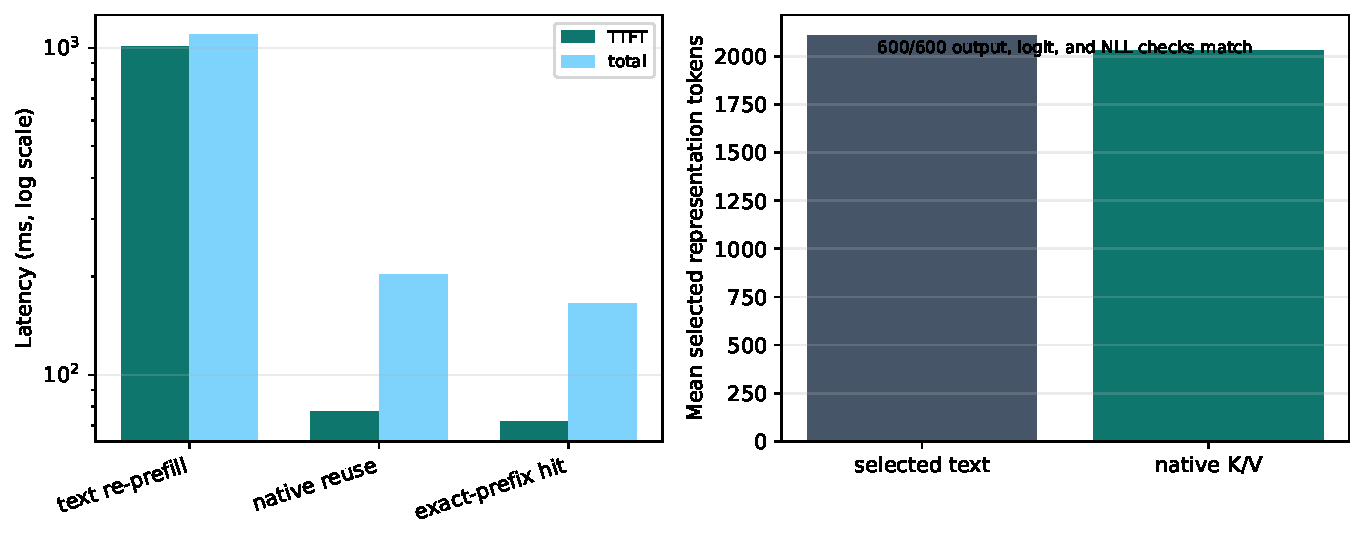
\includegraphics[width=.98\linewidth]{../shared/results/paper3_2_rag/publication/transport_systems_summary.pdf}
\caption{Transport and systems result. Warm native reuse removes evidence
re-prefill while preserving all measured outputs, logits, and NLLs. Exact-prefix
caching remains faster for an unchanged serialized prefix.}
\label{fig:transport}
\end{figure}

Relative to text re-prefill, warm native reuse reduces TTFT by 92.3\% and total
latency by 81.5\%. Cold native execution is 0.8\% slower in TTFT and 3.7\%
slower end to end. An exact prefix hit is 6.9\% faster in TTFT and 18.9\%
faster in total latency than warm native reuse. Native transport does not beat
a perfect exact-prefix cache.

In 25 four-turn sequences with changing selections, ordinary exact-prefix
caching reuses zero evidence tokens. PRA reuses 372.1 of 1325.0 selected K/V
entries per turn (28.1\%) and reduces measured total time from 716.6 to
557.6~ms (22.2\%). This establishes non-prefix addressability, not quality-safe
composition: unrepaired rebound reaches .172 F1 versus .217 for fresh packing.

\begin{figure}[t]
\centering
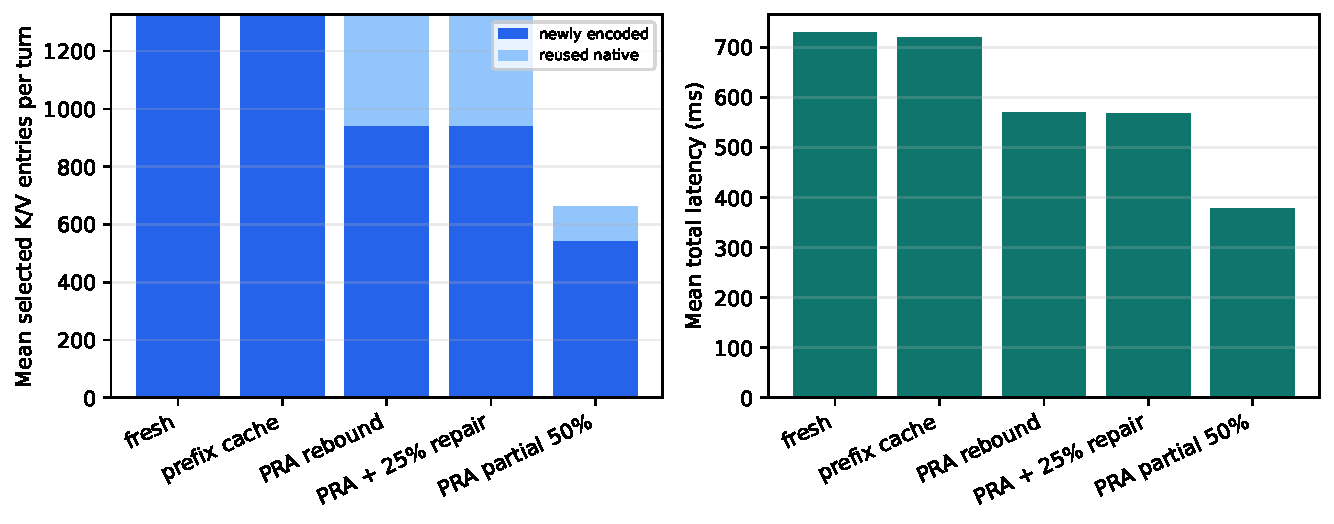
\includegraphics[width=.95\linewidth]{../shared/results/paper3_2_rag/publication/nonprefix_reuse.pdf}
\caption{Changing-selection sessions. Exact-prefix reuse is zero, while PRA
reuses resource-addressed K/V. Partial disclosure saves more work but does not
preserve quality.}
\label{fig:nonprefix}
\end{figure}
\FloatBarrier

\section{Result II: Independent Records Lose Causal Context}
\label{sec:composition}

The central experiment holds token sequence, separators, order, query, and
packed positions fixed while changing the document attention graph. A is full
packed causal RAG. B prevents document tokens from attending across documents,
while query tokens see all documents. C encodes each record independently and
applies B's exact packed positions at request time.

\begin{table}[t]
\centering
\caption{Five-seed causal decomposition. JS uses A as reference for B and B as
reference for C, matching each intervention.}
\label{tab:decomposition}
\small
\begin{tabular}{lrrrr}
\toprule
Condition & Token F1 & Official & Gold NLL & First-step JS \\
\midrule
A: full causal packed & .1187 & .467 & 5.940 & -- \\
B: packed, cross-doc blocked & .1103 & .400 & 3.486 & .1601 vs A \\
C: independent, exact offsets & .1081 & .393 & 3.474 & .00088 vs B \\
\bottomrule
\end{tabular}
\end{table}

C nearly reproduces B at task level: F1 differs by .0022 and first-step JS is
$8.80\times10^{-4}$. The larger change occurs between A and B, where
cross-document causal contextualization is removed. Position is not irrelevant;
it is simply not the missing interaction.

\begin{figure}[t]
\centering
\begin{minipage}{.49\linewidth}
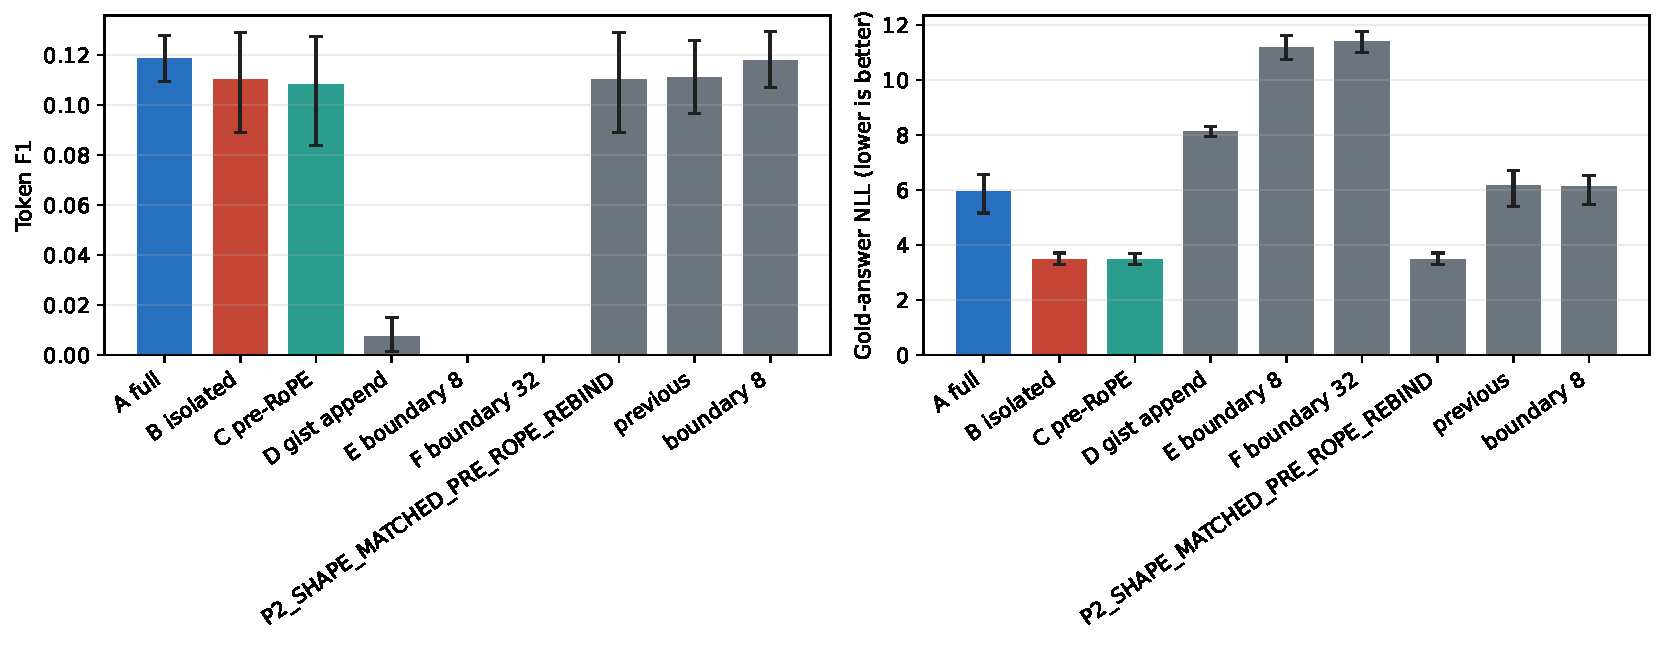
\includegraphics[width=\linewidth]{../shared/results/paper3_2_rag/crossdoc_composition/natural/five_seed/causal_decomposition_quality.pdf}
\end{minipage}\hfill
\begin{minipage}{.49\linewidth}
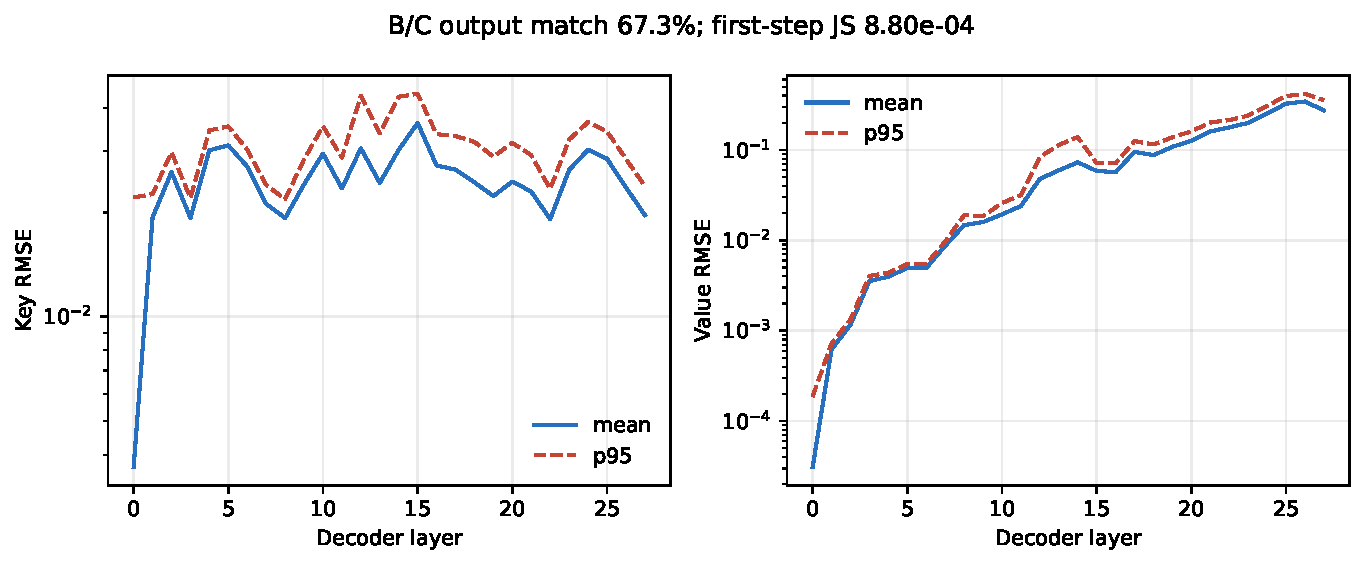
\includegraphics[width=\linewidth]{../shared/results/paper3_2_rag/crossdoc_composition/natural/five_seed/bc_layer_fidelity.pdf}
\end{minipage}
\caption{Causal decomposition. Left: removing cross-document edges changes
quality; parameter-free repair does not recover it. Right: small B/C numerical
differences grow through the quantized decoder.}
\label{fig:causal}
\end{figure}

A stricter P2 control retains pre-RoPE keys inside B's single packed tensor and
reapplies host RoPE without changing segmentation, projection shape, or
attention shape. P2 is exact at FP32, FP16, INT8, and INT4. Separately shaped
B/C execution has small early-layer differences that grow through the 4-bit
decoder, yielding 67.3\% output agreement. Rebinding and numerical shape-path
qualification are separate gates; neither reconstructs A's causal history.

Order controls reinforce this conclusion. With selected identities fixed,
canonical, reverse, and random packing change behavior because causal document
history changes. Independent records are less order-sensitive because they
remove those edges, but lower sensitivity is not a quality win by itself.
\FloatBarrier

\section{Result III: Composition Repair Frontier}
\label{sec:repair}

Score-ranked 75\% disclosure reduces active K/V from 1320.4 to 990.3 and TTFT
from 88.2 to 68.6~ms, but F1 falls from .234 to .181. Smaller budgets are
non-monotonic. An equal-budget evidence oracle improves support coverage at
25\% (.393 versus .318) but not full-context F1; wrong memory reduces support
coverage to .132. This is a \negative{} fixed-policy result.

\begin{figure}[t]
\centering
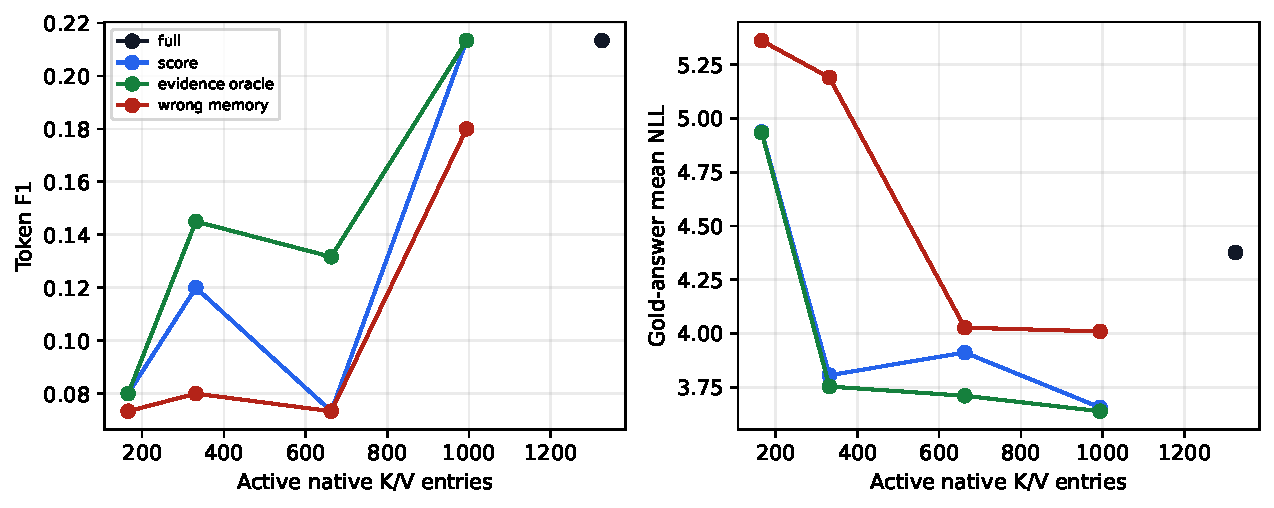
\includegraphics[width=.96\linewidth]{../shared/results/paper3_2_rag/publication/partial_materialization_frontier.pdf}
\caption{Partial-materialization frontier. F1 and NLL are non-monotonic in
active K/V; evidence coverage and generated behavior cannot be inferred from
token count alone.}
\label{fig:partial}
\end{figure}

Appending one mean K/V gist per record, adding all-to-all gist interaction, or
copying 8 or 32 boundary tokens uses only 4--256 ephemeral tokens and 16--272
request-specific interactions. Yet mean F1 falls from .108 for independent
pre-RoPE records to .007, .000, and .000. Fixed sparse document interaction is
also non-monotonic. More interaction is not sufficient; added state must be
calibrated to the frozen decoder.

\begin{figure}[t]
\centering
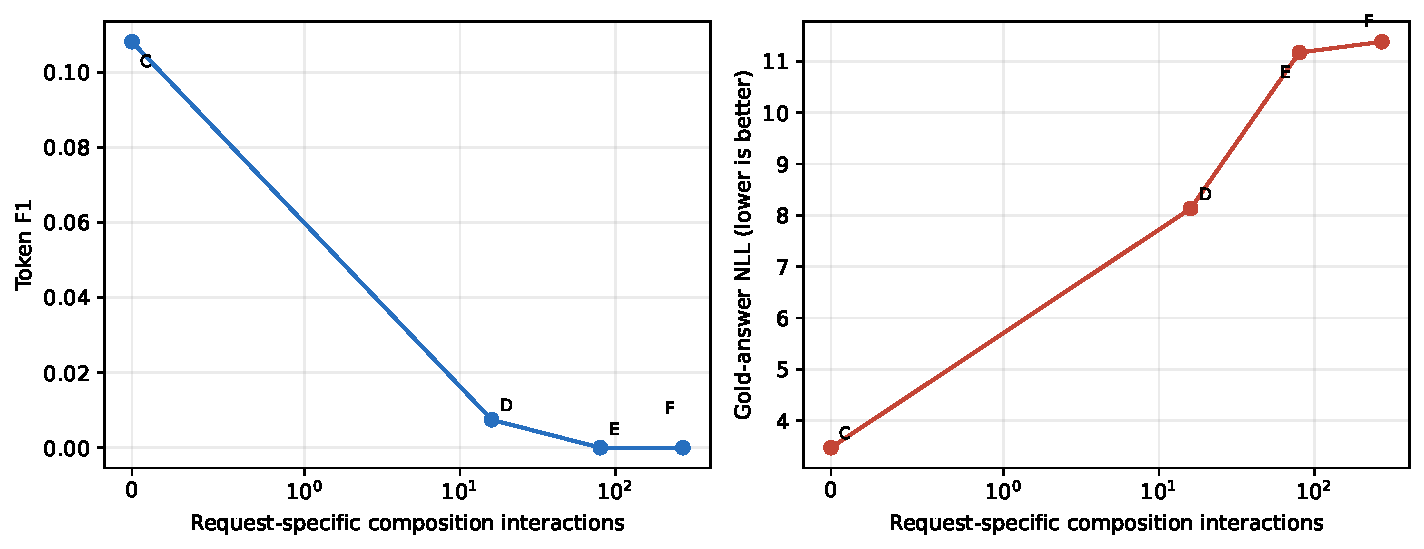
\includegraphics[width=.90\linewidth]{../shared/results/paper3_2_rag/crossdoc_composition/natural/five_seed/gist_composition_frontier.pdf}
\caption{Parameter-free gist and boundary composition. More request-specific
interactions sharply degrade F1 and NLL. Arbitrary synthetic K/V is not a safe repair.}
\label{fig:gist}
\end{figure}

A zero-initialized rank-8 residual (1.38M parameters) is trained on 12 examples
from three seeds and evaluated on 30 disjoint examples across five new seeds.
It raises F1 from .1352 to .1535 and official score from .433 to .533, while
first-step JS falls from .1509 to .0907. However, its paired F1 change of
+.0183 has interval $[-.0136,.0558]$, NLL worsens from 2.929 to 3.330, and
packed RAG remains at .1986 F1 and .700 official score.

Selective boundary re-encoding is the nonparametric comparator. Re-encoding
16 boundary tokens per record reaches .1525 F1, but official score stays .433,
NLL worsens to 5.178, and request transformation costs 191~ms. Neither method
passes a joint generation, likelihood, and systems gate.

\begin{figure}[t]
\centering
\begin{minipage}{.56\linewidth}
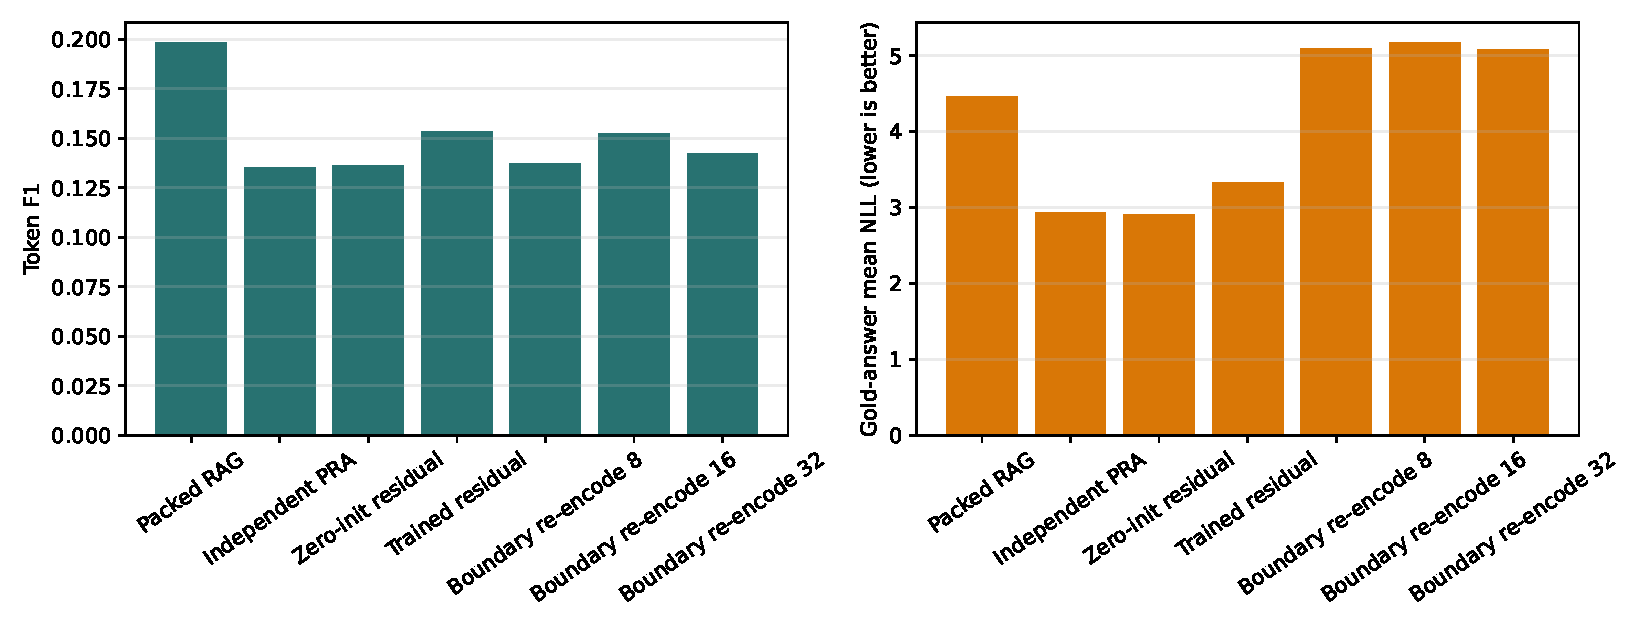
\includegraphics[width=\linewidth]{../shared/results/paper3_2_rag/crossdoc_adapter/qwen3_1_7b_rank8_five_seed/crossdoc_adapter_quality.pdf}
\end{minipage}\hfill
\begin{minipage}{.42\linewidth}
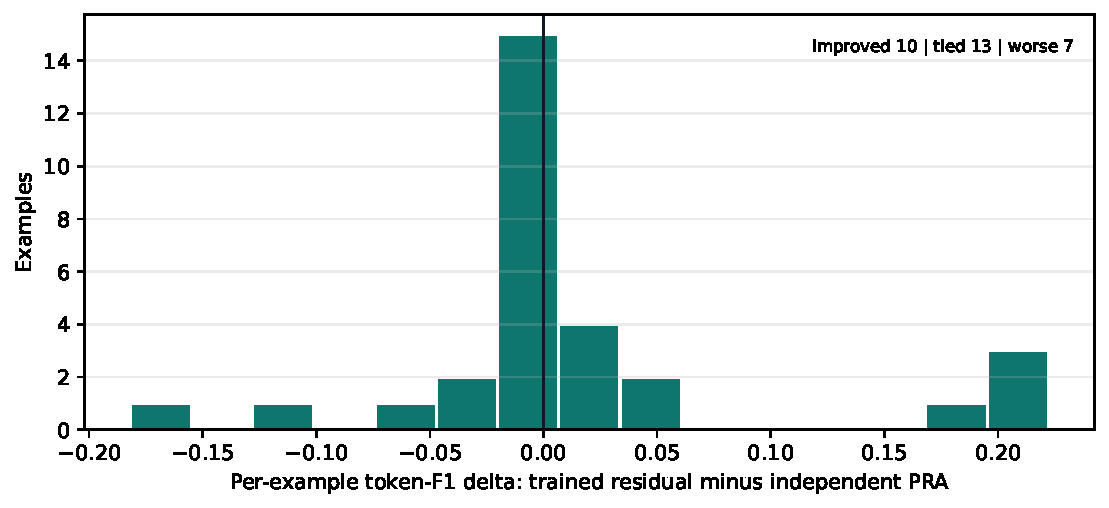
\includegraphics[width=\linewidth]{../shared/results/paper3_2_rag/publication/adapter_f1_delta_histogram.pdf}
\end{minipage}
\caption{Learned-repair frontier. Aggregate F1 improves while NLL worsens and
packed RAG remains stronger (left). Per-example deltas show 10 improvements,
13 ties, and 7 regressions (right); seed-level uncertainty governs the claim.}
\label{fig:adapter}
\end{figure}

\begin{table}[t]
\centering
\caption{Representative held-out repair frontier.}
\label{tab:repair}
\small
\begin{tabular}{lrrrrr}
\toprule
Condition & F1 & Official & NLL & JS & Re-encoded \\
\midrule
Packed RAG & .1986 & .700 & 4.467 & .0000 & 0 \\
Independent PRA & .1352 & .433 & 2.929 & .1509 & 0 \\
Trained rank-8 residual & .1535 & .533 & 3.330 & .0907 & 0 \\
Boundary re-encode 16 & .1525 & .433 & 5.178 & .0876 & 40 \\
Boundary re-encode 32 & .1424 & .467 & 5.077 & .0795 & 80 \\
\bottomrule
\end{tabular}
\end{table}

\subsection{Protocol reconciliation: the gap is budget-dependent}

The repair cohort above used the earlier BM25-v1 implementation, 256-token
chunks, a 1,024 model-token budget, and chunk-level selection. Paper 3.3 used
corrected deterministic BM25-v2, 128-token chunks, one chunk per document, and
about 512 source tokens. Their reported .700 and .427 packed scores therefore
were not repeated measurements of one protocol.

We reran both historical cohorts with Qwen3-1.7B-4bit revision
\texttt{3b1b1768}, BGE-v2-M3 revision \texttt{953dc6f6}, one prompt and
evaluator, and one frozen selection receipt per packed/PRA pair. All 150
Paper 3.3 512-token selections reproduce the published anchor, and all 390
packed/PRA pairs share their receipt. No new PRA mechanism is introduced.

\begin{table}[t]
\centering
\caption{Protocol-locked reconciliation. $\Delta$ is independent PRA minus
packed RAG; intervals are paired 10,000-sample bootstrap intervals. The legacy
row budgets model-native tokens; the other rows budget source whitespace
tokens.}
\label{tab:protocol-reconciliation}
\small
\resizebox{\linewidth}{!}{\begin{tabular}{lrrrrrr}
\toprule
Cohort / budget & $n$ & Packed Off. & PRA Off. & $\Delta$ Off. [95\% CI] & Packed F1 & PRA F1 \\
\midrule
Paper 3.3 test, 512 & 150 & 0.427 & 0.433 & +0.007 [-0.073,+0.087] & 0.086 & 0.090 \\
Paper 3.3 test, 1,024 & 150 & 0.527 & 0.333 & -0.193 [-0.280,-0.107] & 0.087 & 0.057 \\
Paper 3.2 eval, 512 & 30 & 0.433 & 0.333 & -0.100 [-0.267,+0.067] & 0.085 & 0.081 \\
Paper 3.2 eval, 1,024 & 30 & 0.533 & 0.333 & -0.200 [-0.333,-0.067] & 0.101 & 0.080 \\
Paper 3.2 legacy-v2 & 30 & 0.567 & 0.500 & -0.067 [-0.300,+0.167] & 0.102 & 0.103 \\
\bottomrule
\end{tabular}
}
\end{table}

At the exact Paper 3.3 512-token endpoint, independent PRA is indistinguishable
from packed RAG: official score differs by +.007
($[-.073,.087]$) and F1 by +.003 ($[-.010,.017]$). Doubling the common budget
materializes about 1,012 source tokens (1,335 model-native tokens). Packed
official score rises by .100 ($[.027,.173]$), while independent PRA changes by
-.100 ($[-.167,-.033]$). The resulting independent-minus-packed gap is $-.193$
($[-.280,-.107]$), with F1 $-.030$ ($[-.046,-.015]$). More selected
source-local state is not monotonically more useful to the frozen decoder.

The old 30 identities show the same common-protocol trend: packed scores .433
at 512 and .533 at 1,024, while independent PRA remains .333. Cohort
composition therefore does not explain the packed endpoint difference by
itself. Replaying the exact legacy geometry with BM25-v2 changes 14 of 30
selections (mean chunk-set Jaccard .713) despite nearly identical token use.
Packed score falls from the reported .700 to .567; independent PRA rises from
.433 to .500. Their corrected gap is $-.067$ ($[-.300,.167]$), and F1 is tied
at .102 versus .103. BM25-v1 to v2 reduces packed F1 by .097
($[-.127,-.069]$) and independent F1 by .033 ($[-.051,-.011]$).

\begin{figure}[t]
\centering
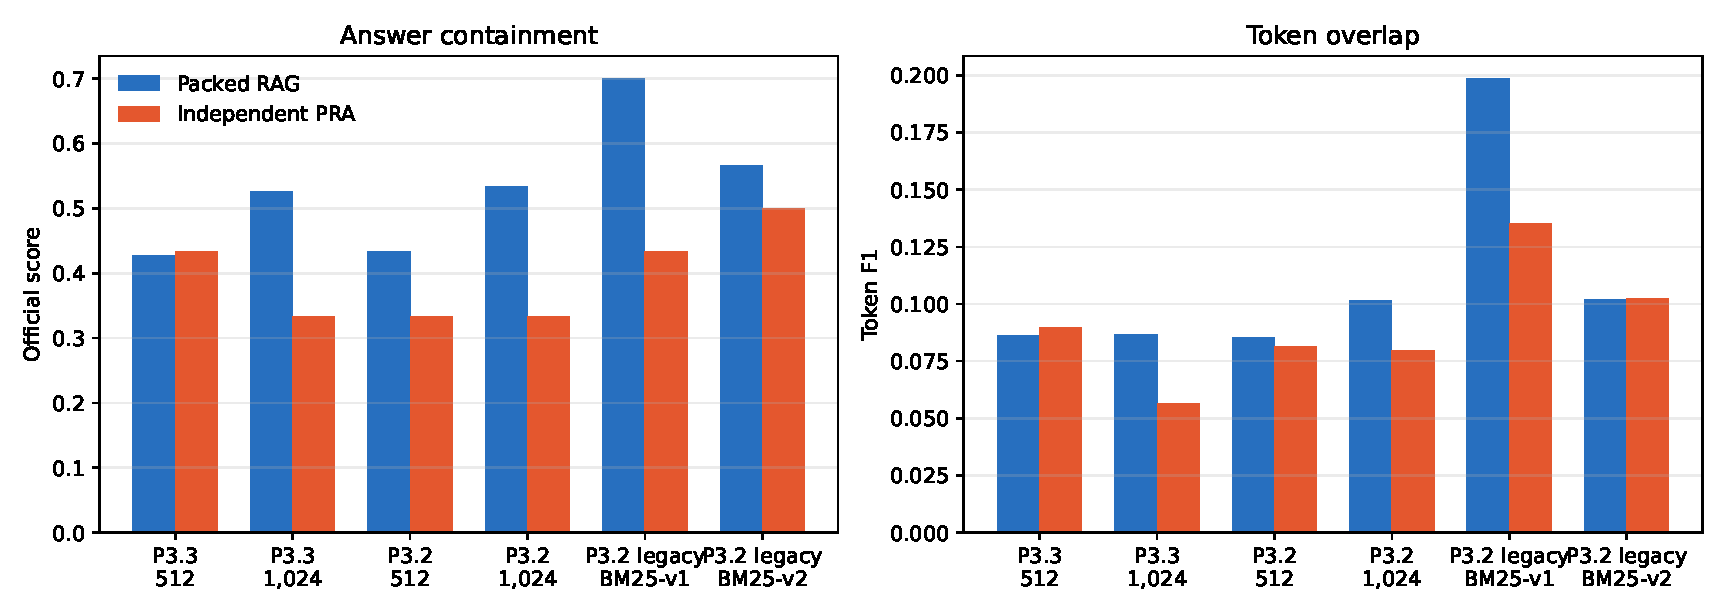
\includegraphics[width=\linewidth]{../shared/results/paper3_2_rag/protocol_reconciliation/protocol_reconciliation.pdf}
\caption{Matched reconciliation. The 512-token Paper 3.3 endpoint is a parity
result; the larger common budget favors causal packing. Correcting BM25 under
the legacy Paper 3.2 geometry removes most of the reported packed advantage.}
\label{fig:protocol-reconciliation}
\end{figure}
\FloatBarrier

\section{Discussion}

\paragraph{Persistent K/V is contextual state, not document content.}
Contiguous transport succeeds because it preserves state from the same causal
computation. Packed documents have directed edges
$D_1\rightarrow D_2\rightarrow D_3\rightarrow Q$; independent records meet
only at $Q$. Matching RoPE coordinates does not insert missing arrows.

\paragraph{Retrieval and realization are orthogonal.}
PRA need not replace BM25, FAISS, Elasticsearch, Qdrant, a hybrid retriever, or
a cross-encoder. Retrieval metrics cannot substitute for transport parity, and
transport parity cannot excuse weak selection.

\paragraph{The opportunity begins beyond exact prefixes.}
An exact prefix hit is the stronger baseline for an unchanged serialized
prefix. PRA's distinct capability is query-addressed reuse when documents recur
under changed questions, orders, or combinations. The current independent
representation exposes such reuse. It matches packed quality around the
512-source-token endpoint, but the matched 1,024-token audit shows that simply
adding more independent state does not preserve the benefit of causal packing.

The evidence motivates a two-part design:
\[
\text{persistent intrinsic state}+\text{cheap request-dependent contextualization}.
\]
The second term may be learned sparse interaction, selective recomputation, or
another bounded adapter. It must pass generation, likelihood, causal, and
systems checks together; likelihood proximity alone is insufficient.

\section{Limitations}

The principal composition study uses one 1.7B 4-bit family on bounded natural
cohorts. Larger Qwen and Llama experiments are pilots. Separately shaped
low-precision execution remains non-identical even though shape-matched
rebinding passes. The learned repair has little training data and its five-seed
F1 interval crosses zero. Fixed policies do not exhaust all sparse methods.
The protocol audit covers one 150-question split and the earlier 30 identities;
its paired bootstrap samples questions, not model families. Increasing the
budget also increases the selected record set, so it tests the complete frozen
selection policy rather than token count alone. Finally, selector freezing
intentionally isolates realization from retrieval; it does not show that PRA
retrieval beats strong RAG or prove a universal theorem.

\section{Conclusion}

Frozen RAG-selected text can be transported into persistent native K/V without
changing behavior when its causal context is preserved: all 600 measured pairs
match in output, logits, and answer NLL. This gives large warm reuse benefits
relative to re-prefill and non-prefix reuse where exact-prefix caching cannot
match. Independently encoded records are different. RoPE rebinding restores
position but not cross-document context that never occurred. Fixed and
parameter-free repairs fail; a small learned residual shows uncertain headroom.
The protocol-locked audit places that limitation: independent PRA and packed RAG
are statistically indistinguishable near 512 selected source tokens, whereas
packed causal composition wins significantly near 1,024. Corrected BM25-v2 also
removes most of the historical .700-versus-.433 gap under the legacy geometry.
Persistent contiguous transport is established in the measured setting. Cheap,
quality-preserving composition at larger selected contexts remains open.

\bibliographystyle{plain}
\bibliography{../shared/references}

\appendix

\section{Full Retrieval Study}
\label{app:retrieval}

The selector-frozen contract accepts local BM25, hashed dense, FAISS/BGE,
reciprocal-rank fusion, BGE and cross-encoder rerankers, Elasticsearch BM25,
Qdrant/BGE, and a service hybrid. The service hybrid reaches .852 supporting
document Recall@20; Qdrant/BGE reaches .743 and Elasticsearch .735. These
qualify candidate generation, not native realization.

\begin{figure}[h]
\centering
\begin{minipage}{.49\linewidth}
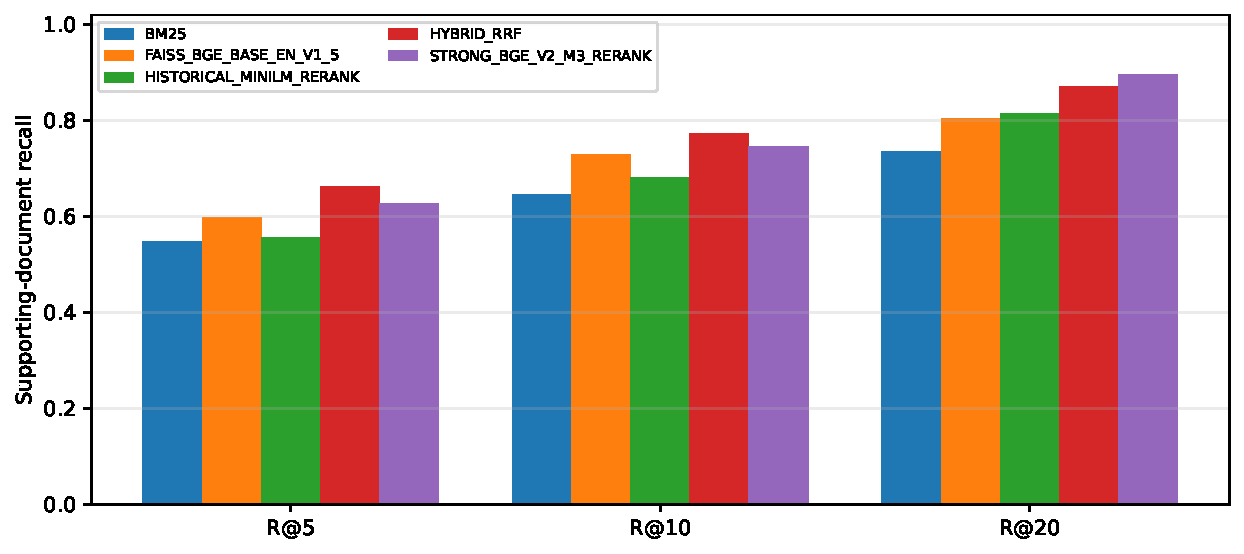
\includegraphics[width=\linewidth]{../shared/results/paper3_2_rag/publication/local_retrieval_recall.pdf}
\end{minipage}\hfill
\begin{minipage}{.49\linewidth}
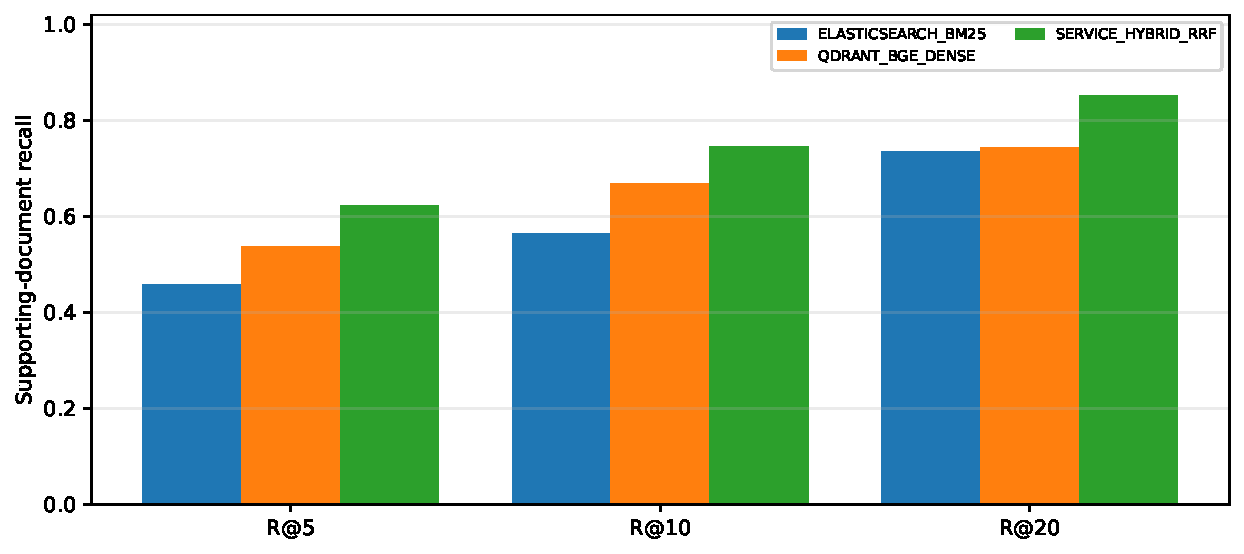
\includegraphics[width=\linewidth]{../shared/results/paper3_2_rag/publication/service_retrieval_recall.pdf}
\end{minipage}
\caption{Local (left) and service-backed (right) retrieval ladders.}
\label{fig:retrieval}
\end{figure}

Service latency is decomposed into embedding, search, and client overhead.
Elasticsearch averages 11.5~ms, Qdrant/BGE 23.4~ms including embedding, and
service hybrid RRF 53.1~ms on the 50-question cohort. The full report retains
backend versions, index revisions, and extended tables.

\section{Dataset, Cohorts, and Statistics}
\label{app:cohorts}

The dataset revision is
\texttt{fcb9efe65c7730dd4126a42afb6c2c7e45721ebb}; the corpus revision is
\texttt{bb98345ef3921312aad05fd117b5a3e39888de2c}. Transport uses five
independently sampled 30-question cohorts. Repair calibration and evaluation
are disjoint. The residual trains on 12 examples associated with seeds 11, 23,
and 37 and evaluates on 30 different examples associated with seeds 131, 151,
181, 211, and 223.

Each seed-cohort mean is one statistical unit. Bootstrap intervals resample the
five seed means 10,000 times with a fixed random seed. Raw or compressed
per-example rows remain committed beside each manifest.

\section{Full Transport and Cache Controls}
\label{app:transport}

The 600 pairs comprise 300 generic-selector and 300 strong-reranker comparisons.
The reduced 4B/8B/family study adds 120 exact pairs. At 4B, Qwen-8B, and
Llama-8B, warm native TTFT is 6.5\%, 5.9\%, and 6.0\% of text re-prefill, but
7.2\%, 4.6\%, and 5.0\% slower than exact-prefix reuse. These scale rows are
\pilot{} because each uses one 20-question cohort.

\begin{figure}[h]
\centering
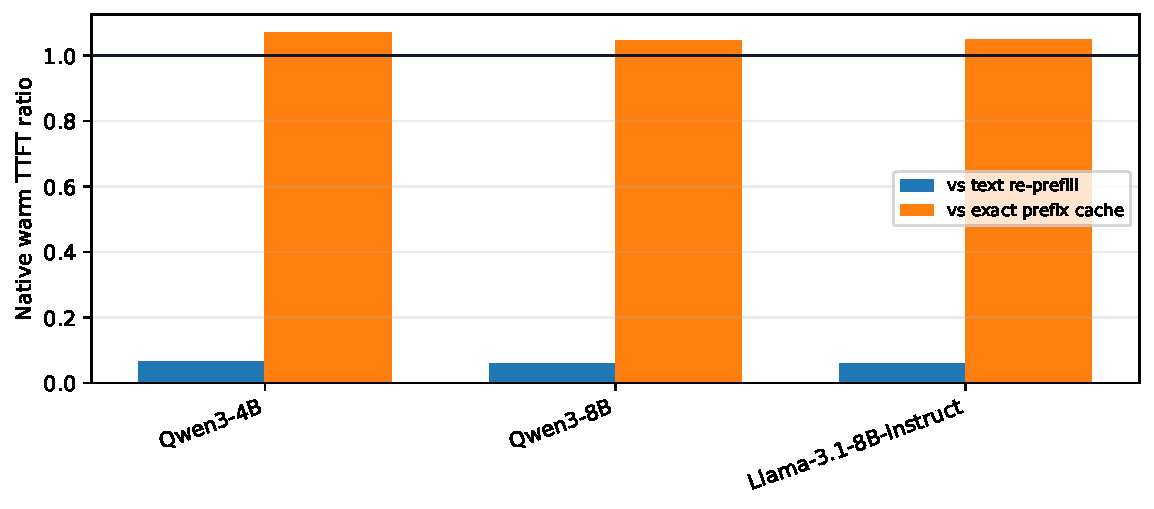
\includegraphics[width=.78\linewidth]{../shared/results/paper3_2_rag/publication/scale_transport.pdf}
\caption{Cross-scale transport pilot. Native reuse is far cheaper than
re-prefill but slightly slower than a perfect prefix hit.}
\label{fig:scale-transport}
\end{figure}

\section{Positional Transport and Precision}
\label{app:rope}

The runtime captures projected keys before host RoPE and keeps values
unchanged. P2 changes only storage/rebinding and is exact at FP32, FP16, INT8,
and INT4. Separately shaped record projection and attention calls introduce
precision-dependent drift that compounds by layer.

\begin{figure}[h]
\centering
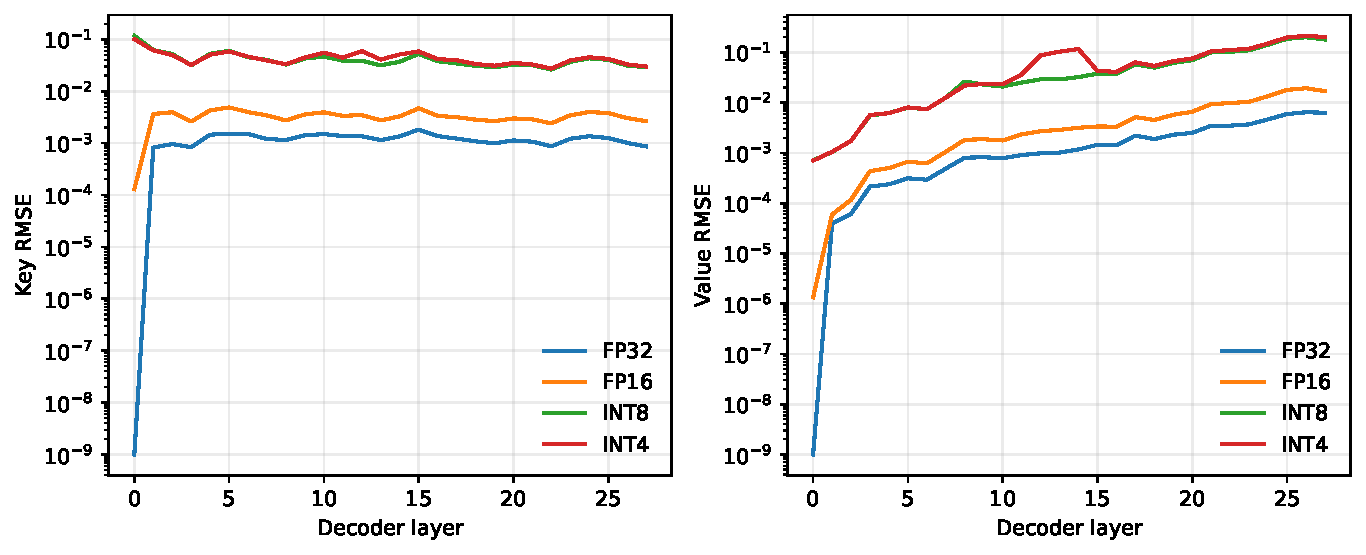
\includegraphics[width=.82\linewidth]{../shared/results/paper3_2_rag/crossdoc_precision/aggregate/precision_layerwise_rmse.pdf}
\caption{Layerwise B/C precision diagnostic. Shape-matched rebinding is exact;
separate record-wise execution introduces drift.}
\label{fig:precision}
\end{figure}

The initial Llama pilot incorrectly assumed one RoPE base and produced JS .526.
The corrected path reads the host layer's piecewise frequency tensor. Only
corrected values appear here.

\section{Independent-Record Diagnostics}
\label{app:composition}

Independent records use the canonical URI-addressed \texttt{ContextRecord} and
resolver path. Explicit and rooted references agree exactly, excluding parser
or root resolution as the measured loss. Stronger selectors improve evidence
coverage, but independent realization remains below packed RAG in replicated
1.7B and 4B studies.

\begin{figure}[h]
\centering
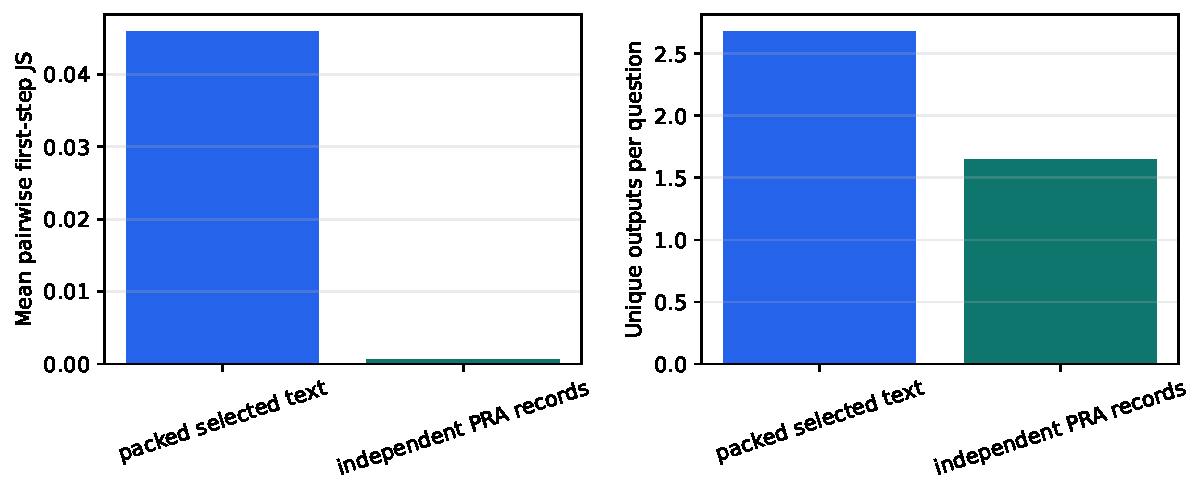
\includegraphics[width=.85\linewidth]{../shared/results/paper3_2_rag/publication/native_record_order_sensitivity.pdf}
\caption{Packed and independent-record order sensitivity. Reduced sensitivity
from removing cross-document edges is not itself a quality gain.}
\label{fig:order}
\end{figure}

Canonical, reverse, and seeded-random orders freeze identities and content.
Packed results vary because causal history varies; independent records vary less
because documents meet only at the query.

\section{Partial Materialization and Sparse Interaction}
\label{app:partial}

Score, evidence-oracle, and wrong-memory policies are evaluated at 12.5\%,
25\%, 50\%, and 75\%. None gives a monotonic F1/NLL frontier. Fixed masks include
previous-document, top-ranked-to-all, and 8/16/32/64-token boundaries. The
eight-token window uses 99.97\% fewer cross-document edges than full packing and
approaches its mean F1, but fails official-score and NLL gates.

A diagnostic 25\% repair raises changing-selection output recovery to 44\% but
requires 1284.1 newly encoded or recomputed states, only 3.1\% less than fresh
packing. Partial 50\% disclosure cuts new work by 57.1\% and measured time by
47.2\%, but reaches only .150 F1 and 6\% parity.

\section{Parameter-Free Repair Attempts}
\label{app:fixed}

The family includes mean K/V gists, all-to-all gist mixing, first/last boundary
copies, and request-local 8- or 32-token windows. It never overwrites persistent
records and uses one host attention normalization over persistent, ephemeral,
and query state. Every variant fails the five-seed gate and reduced Qwen/Llama
pilots. This rules out a tempting shortcut: arbitrary synthetic K/V is not
automatically meaningful to a frozen decoder.

\section{Learned Residual Repair}
\label{app:learned}

The rank-8 adapter is zero-initialized and optimized for 100 AdamW steps at
$2\times10^{-4}$ with K/V distillation, response distillation, and 0.1 task-loss
weight. The paired F1 deltas versus independent PRA are +.0633 for packed RAG
([.0264,.1170]), +.0183 for the trained residual ([-.0136,.0558]), +.0173 for
16-token re-encoding ([-.0230,.0474]), and +.0072 for 32-token re-encoding
([-.0184,.0328]). With five seeds, the trained effect remains \pilot{}.

\begin{figure}[h]
\centering
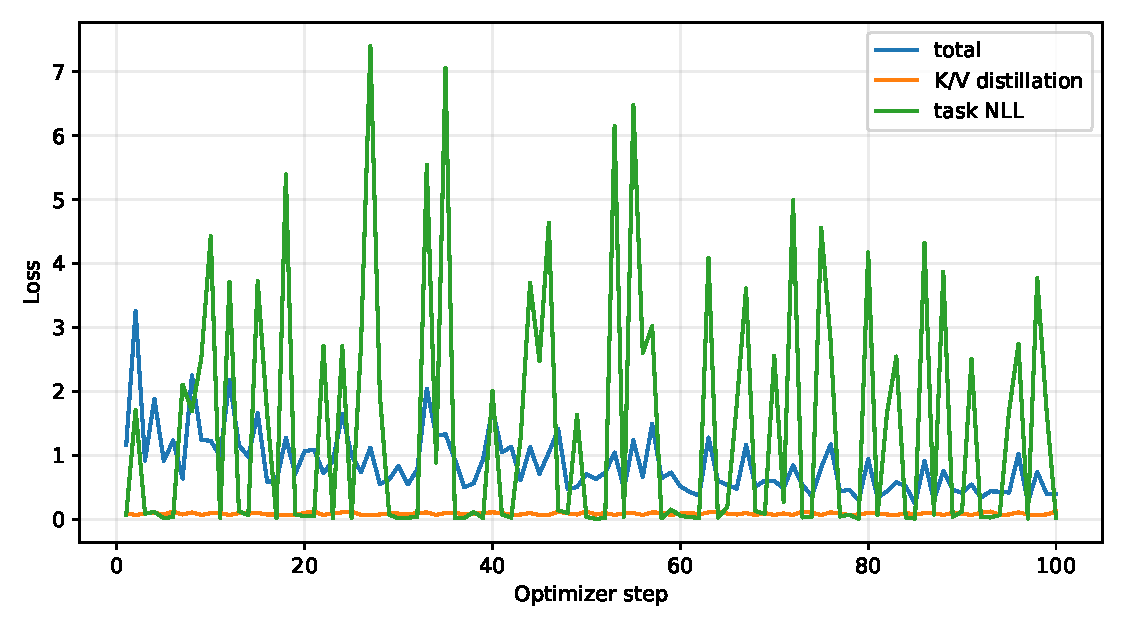
\includegraphics[width=.76\linewidth]{../shared/results/paper3_2_rag/crossdoc_adapter/qwen3_1_7b_rank8_five_seed/crossdoc_adapter_training.pdf}
\caption{Residual calibration history. Step 100 is selected; evaluation data
and seeds are disjoint from calibration.}
\label{fig:adapter-training}
\end{figure}

\section{Cross-Model Pilots}
\label{app:scale}

On five questions in canonical and reverse order, 50\% later-resource prefix
repair recovers 8/10 Qwen3-4B, 5/10 Qwen3-8B, and 7/10 Llama-3.1-8B outputs.
Packed rebinding alone recovers 2/10, 0/10, and 3/10; full repair reaches 10/10
for all. This does not establish a monotonic scale law.

\begin{figure}[h]
\centering
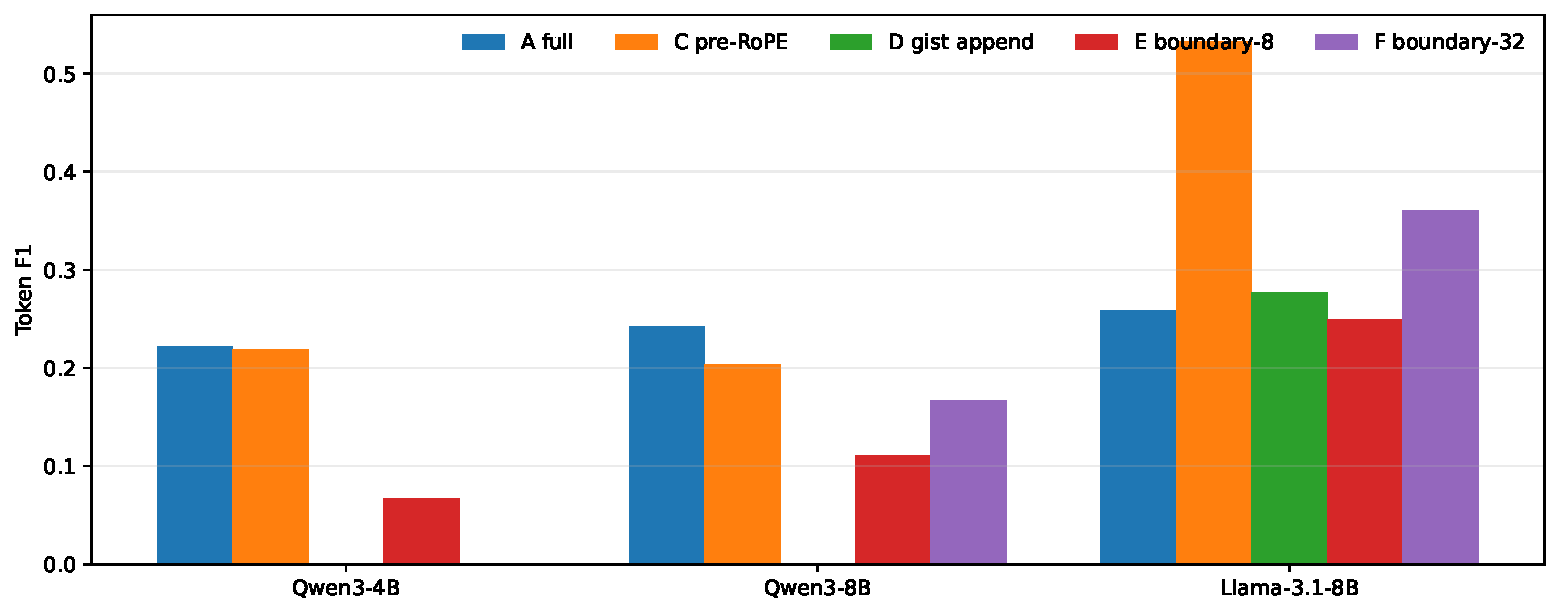
\includegraphics[width=.84\linewidth]{../shared/results/paper3_2_rag/crossdoc_composition/scale/aggregate/crossdoc_scale_quality.pdf}
\caption{Reduced cross-model composition pilot.}
\label{fig:scale-composition}
\end{figure}

\section{Systems, Artifacts, and Evidence Ledger}
\label{app:systems}

Runs persist dataset/corpus revisions, query identity, candidate and selection
receipts, scores, record IDs, spans, order, positions, precision, generation
settings, backend versions, hardware, and commit ID. Native records use immutable
URIs and source hashes. Overlap is deduplicated only within one source domain.

\begin{sloppypar}
The compact entry point is
\path{docs/papers/shared/results/paper3_2_rag/publication/publication_summary.json}.
Figures are regenerated by
\path{experiments/paper3_2_rag/build_publication_artifacts.py}. The exhaustive
experimental sequence, configurations, and tables remain in
\texttt{paper\_3\_2\_full.pdf}.
\end{sloppypar}

\begin{table}[h]
\centering
\caption{Evidence hierarchy after reorganization.}
\small
\begin{tabular}{p{.20\linewidth}p{.70\linewidth}}
\toprule
Status & Result \\
\midrule
Established & 600/600 contiguous checks; shape-matched host-RoPE rebinding; exact-prefix and changing-selection cache controls \\
Qualified boundary & Independent records track blocked packed context; separately shaped INT4 is approximate; sparse interaction is non-monotonic \\
Negative & Fixed partial materialization; parameter-free gist append; post-hoc boundary copies \\
Pilot / uncertain & 4B/8B and Llama composition; rank-8 residual with interval crossing zero \\
\bottomrule
\end{tabular}
\end{table}

\end{document}
